% !TEX root = ../thesis.tex
\chapter{Results and Discussion}
\label{chap:results}

We will first look at the web application results based on the user's feedback, and then we will look into the insights and potential feedback the NLP process could provide the user. We then also look to review the overall process. 

We will compare the web application's results against the comparative judgment, Elo ranking, and the score we created for the tweets on Twitter. With the insights of the NLP for feedback to the user, we will look at what insights got made. Additionally, we will look at if any of the knowledge extracted generated provides any meaningful feedback to the user.



\section{Tweet Ranking Results} 
\label{sec:reaults_ranking}

\begin{figure}[h]
	\centering
	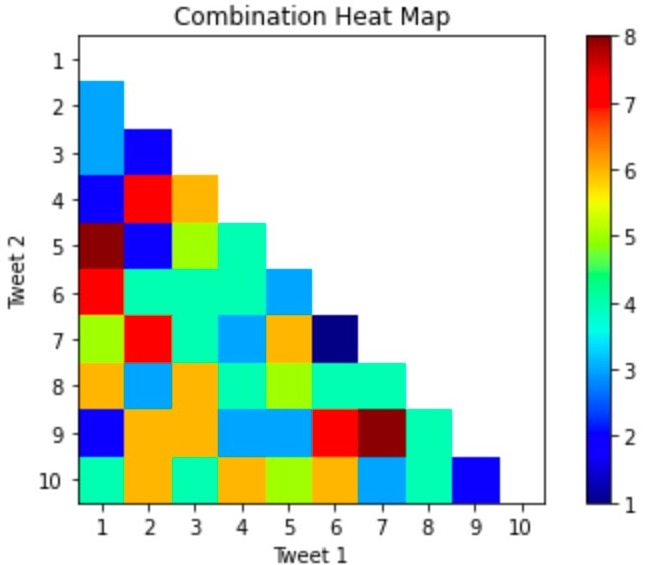
\includegraphics[width=7cm]{combination_heat_map.png}
	\caption{The web applicaitons generated results compared agaist each other.}
	\label{fig:combinations}
	
\end{figure}

Forty different users take part in the comparison judgement within the web app. Through looking at fig: \ref{fig:combinations} we can see that all combinations got displayed to the users taking part in the comparisons. We can see that tweet one and tweet five appeared the most, while the combination appearing the lowest was tweet six and seven, with one comparison getting presented to the users.



When we look at winners and losers of the comparisons( see fig: \ref{fig:combination_wins}), we can see that the tweet that won the most between a specific combination was tweet four and two, with tweet four winning six times and tweet two winning only once. Additionally, when we look at the combination that appeared the most, one and five, one came out on top five times, compared to five winning between the two once.
\begin{figure}[h]
	\centering
	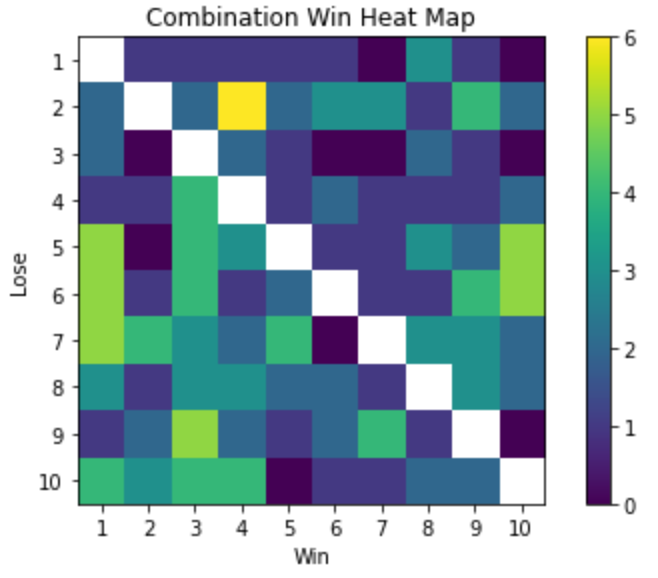
\includegraphics[width=7cm]{combination_win_heat_map.png}
	\caption{A heat map of the amount of times a tweet win or lost}
	\label{fig:combination_wins}
	
\end{figure}

When we look at the winner heat map (see fig: \ref{fig:combination_wins}), we can see that two, five, six, seven and ten had moments where they didn't win a head-to-head with another tweet. Two, six, seven and ten didn't win against at least two different tweets, while the others were only against one tweet they failed to win.


While looking at fig \ref{fig:web_app_results}, we can see that the Elo and comparative judgement ranking generated very similar results. However, as we can see, the tweets coming in 6th, 7th and 8th a slight variation in the results.

\begin{figure}[h]
	\centering
	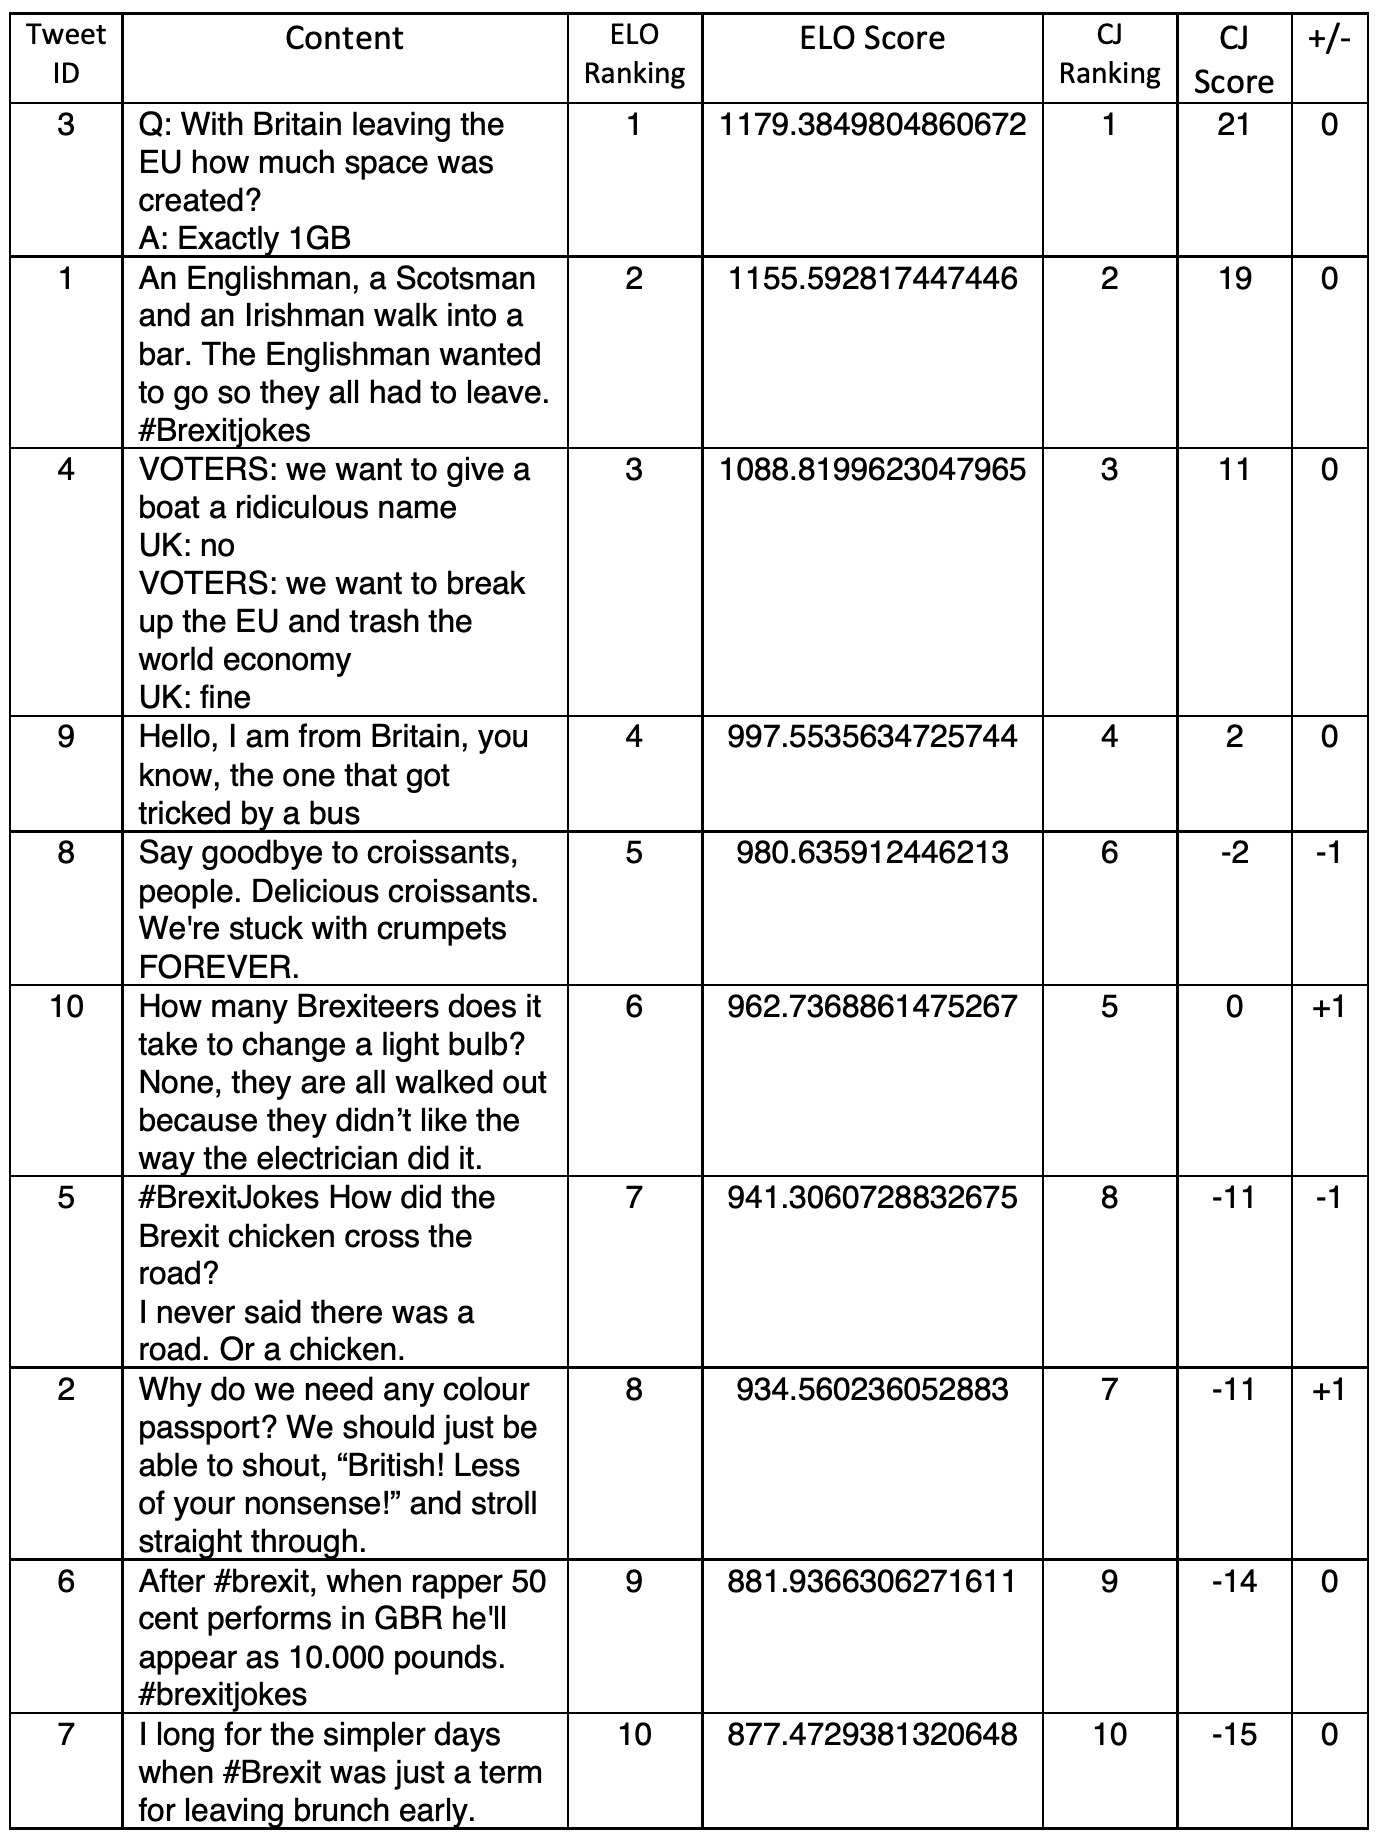
\includegraphics[width=10cm]{web_app_results.png}
	\caption{The web applicaitons generated results compared agaist each other.}
	\label{fig:web_app_results}
	
\end{figure}

\begin{figure}[h]
	\centering
	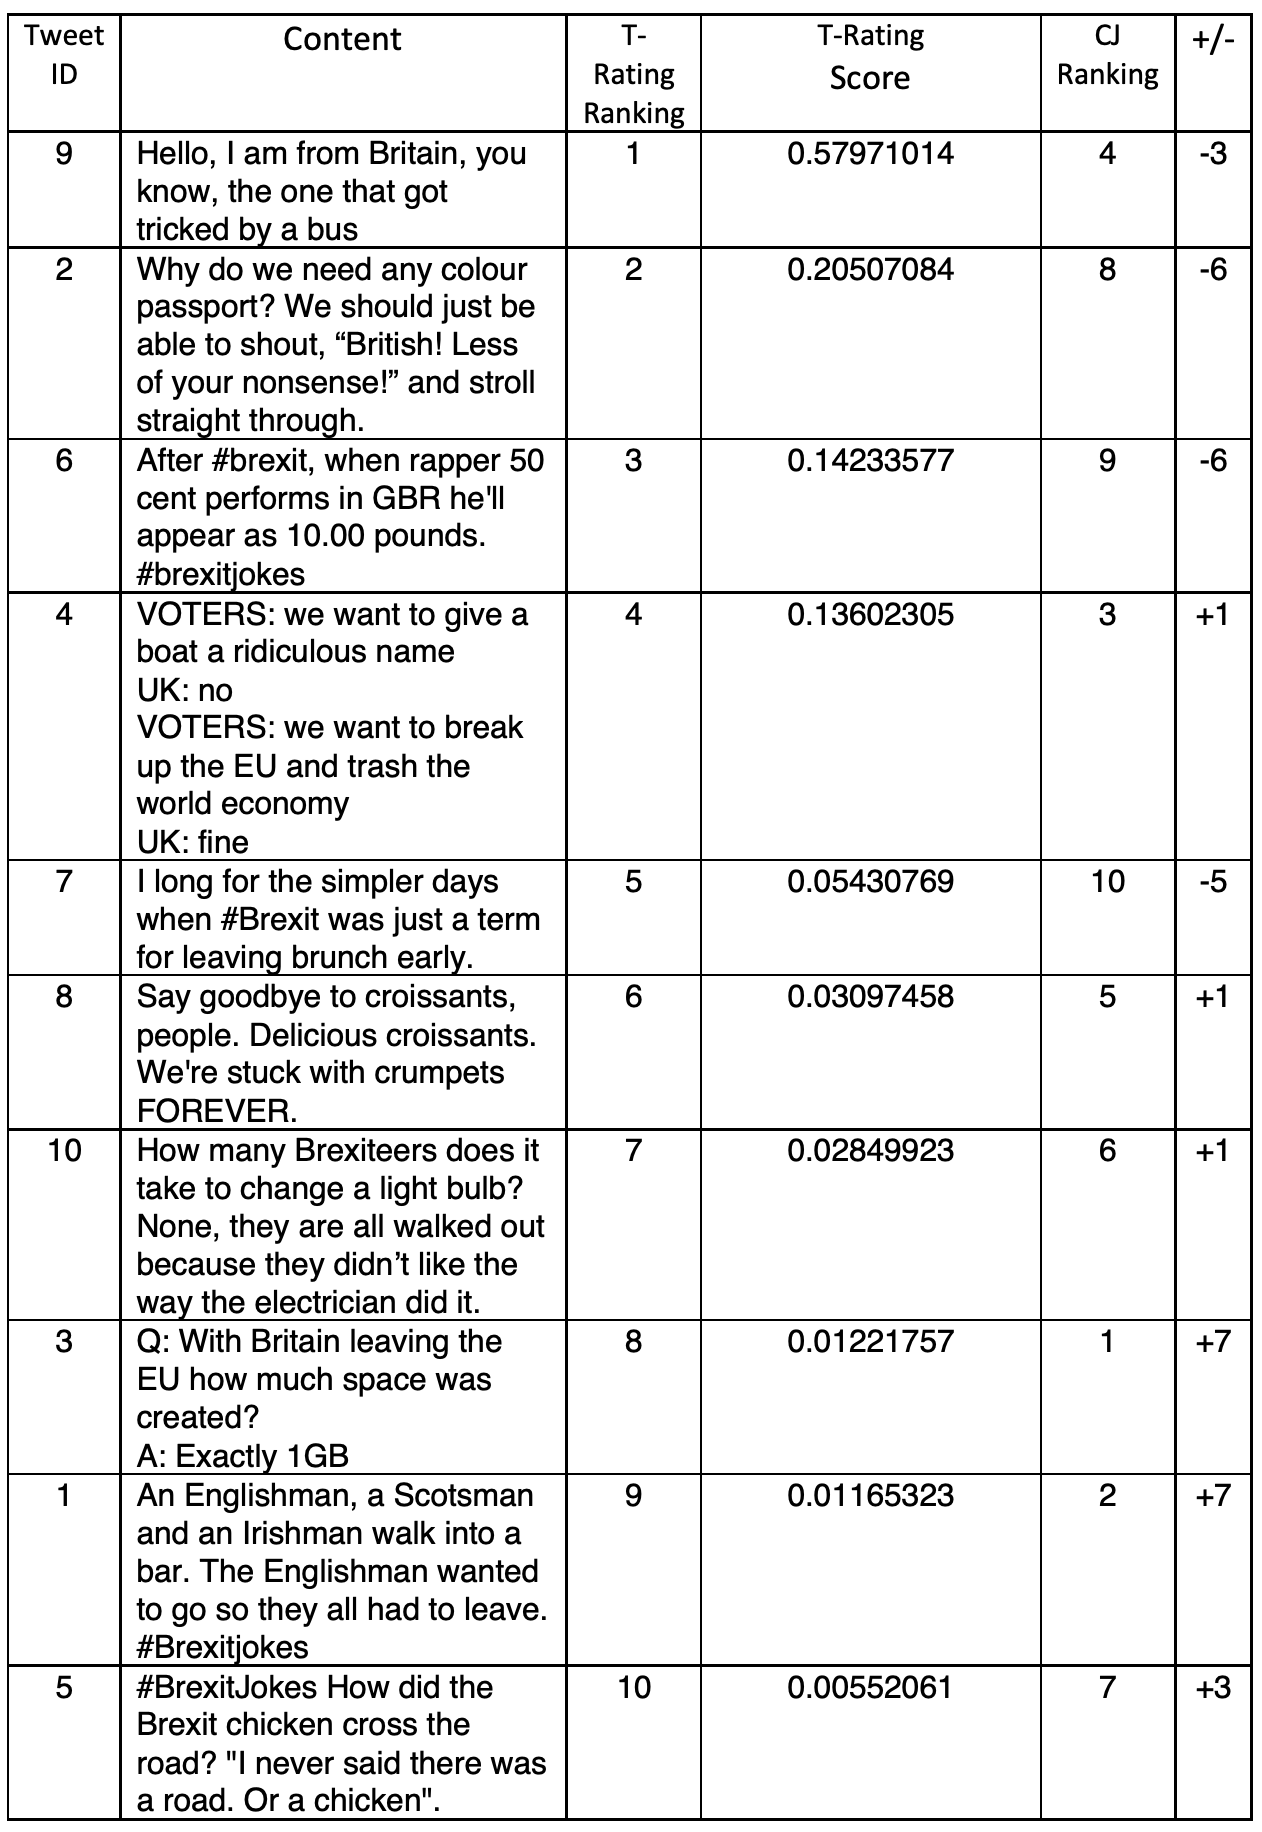
\includegraphics[width=10cm]{twitter_results_comparison.png}
	\caption{The Twitter tweet score ranking comparison against Elo ranking.}
	\label{fig:twitter_results_comparison}
	
\end{figure}



\section{NLP Feedback and Insights}
\label{sec:reaults_NLP}

\section{Overall Results}
\label{sec:reaults_NLP}

